\chapter{物体的平衡}
我们知道,如果已知物体所受的力,根据牛顿第二定律就可以求出这个物体的加速度。
然而知道受力物体在什么条件下不产生加速度,这个问题往往也很重要。
我们知道,一个物体既可以做平动,也可以做转动。
如果一个物体既不做平动,也不做转动,即保持静止,或者做匀速度直线运动或匀速转动,我们就说这个物体处于平衡状态。
要使物体保持\Concept{平衡状态},作用在物体上的力必须满足一定的条件,这个条件叫做\Concept{平衡条件}。

研究物体的平衡很有实际意义,工程技术上的很多物体,例如桥梁、起重机、建筑物等,都要保持平衡状态。
在设计桥梁、起重机、建筑物时,必须分析它们各部分的受力情况,然后根据平衡条件来进行计算,以便确定几何尺寸或选择合适的材料。

\section{在共点力作用下物体的平衡}
受共点力作用的物体在什么条件下才能保持平衡呢?

在两个共点力作用下物体的平衡条件,我们在初中已经学过,并且前面也用过了。
物体受到两个共点力的时候,只有这两个力大小相等方向相反,物体才保持平衡状态。
从力的合成法则知道,这时合力等于零。
可见,在两个共点力作用下物体的平衡条件是这两个力的合力等于零。
\begin{figure}
  \begin{minipage}[b]{0.4\linewidth}\centering
    \includegraphics{6-1a.pdf}
    \subcaption{}\label{fig:6-1a}
  \end{minipage}
  \begin{minipage}[b]{0.2\linewidth}\centering
    \includegraphics{6-1b.pdf}
    \subcaption{}\label{fig:6-1b}
  \end{minipage}
  \caption{}\label{fig:6-1}
\end{figure}

在三个共点力作用下物体的平衡条件又是什么呢?
我们用三个弹簧秤同时拉一个物体,并且使这个物体保持平衡(\cref{fig:6-1a})。
从这三个弹簧秤上分别读出它们对物体的拉力 $F_1$、$F_2$ 和 $F_3$,并作出力的图示(\cref{fig:6-1b})。
先求出其中任意两个力的合力,例如 $F_1$ 和 $F_2$ 的合力 $F$,可以看出力 $F$ 和 $F_3$ 作用在同一直线上,并且大小相等方向相反,它们的合力等于零。
也就是说,力 $F_1$、$F_2$、$F_3$ 的合力等于零。
可见,在三个共点力作用下物体的平衡条件是这三个力的合力等于零。

用实验还可以证明,在三个以上共点力作用下物体的平衡条件也是合力等于零。

因此,我们得到结论:\emph{在共点力作用下物体的平衡条件是合力等于零}。如果用 $F_{\text{合}}$ 表示合力,这个平衡条件可以写成
\[F_{\text{合}}=0.\] 

这个结论其实可以从牛顿第二定律推导出来。
从牛顿第二定律的公式 $F_{\text{合}}=ma$ 知道,只有 $F_{\text{合}}=0$,加速度 $a$ 才等于零,物体才能保持平衡状态。

\begin{Practice}
\begin{question}
  \item 在\cref{chp:Force}\cref{fig:1-21} 所示的情形里,如果物体的重量是 \qty{40}{N},绳子 $a$ 与竖直方向成 \ang{30} 角,绳子 $a$ 和 $b$ 对物体的拉力分别是多大?
  \item 把物体放在光滑的斜面上,并用弹簧把它拉住,如\cref{fig:6-2} 所示。如果物体的质量为 $m$,斜面的倾角为 $\theta$,弹簧对物体的拉力是多大?
  \item \cref{fig:6-3} 是起重机匀速起吊重物时吊钩的受力情况。吊钩受到竖直向上的牵引力 $F_1$ 和两条钢索对它斜向下的拉カ $F_2$ 和 $F_3$。如果两条钢索的夹角为 \ang{60},力 $F_2$ 和 $F_3$ 大小相等,力 $F_1$ 为 \qty{2.0e4}{N},每条钢索对吊钩的拉力是多大?
  \begin{figurehere}
    \begin{minipage}[b]{0.4\linewidth}
      \centering\includegraphics{6-2.pdf}
      \caption{}\label{fig:6-2}
    \end{minipage}
    \begin{minipage}[b]{0.58\linewidth}
      \centering\includegraphics{6-3.pdf}
      \caption{}\label{fig:6-3}
    \end{minipage}
  \end{figurehere}
  \item 掘沟机由两台拖拉机牵引(\cref{fig:6-4}),两条绳索对掘沟机的拉力都是 \qty{2.5e4}{N},绳索间的夹角为 \ang{60},如果拖拉机是匀速行进的,土地的阻力有多大?
  \item 如\cref{fig:6-5} 所示,物体在五个共点力的作用下保持平衡,如果撤去力$F_5$,而保持其余四个力不变,这四个力的合力的大小和方向是怎样的?
\begin{figurehere}
  \begin{minipage}[b]{0.48\linewidth}\centering
    \includegraphics{6-4.pdf}
    \caption{}\label{fig:6-4}
  \end{minipage}
  \begin{minipage}[b]{0.48\linewidth}\centering
    \includegraphics{6-5.pdf}
    \caption{}\label{fig:6-5}
  \end{minipage}
\end{figurehere}
\end{question}
\end{Practice}

\section{力对物体的转动作用}
\subsection{转动}
转动是一种常见的运动。物体在转动的时候,它的各点都做圆周运动,这些圆周的中心在同一直线上,这条直线叫做\Concept{转动轴}。
\begin{figure}
  \includegraphics{6-6.pdf}
  \caption{同一时间内,离转动轴远近不同的各点,通过长度不同的弧}\label{fig:6-6}
\end{figure}

从\cref{fig:6-6} 可以看到,转动物体上离转动轴远近不同的点 $A_1$、$A_2$、$A_3$ 在同一时间内,通过长度不同的弧 $A_1B_1$、$A_2B_2$、$A_3B_3$。
离转动轴越远的点,通过的弧越长,但是连接 $A_1$、$A_2$、$A_3$ 和圆心 $O$ 的半径转过的角度是相等的。
可见,转动物体上离转动轴远近不同的点,线速度不同,而角速度相同。

我们知道,平动物体上各点的速度都相同,任何一点的速度都可以代表整个物体的速度。
同样,转动物体上各点的角速度都相同,任何一点的角速度都可以代表整个物体的角速度。
因此,研究物体的转动,常用角速度表示转动的快慢。

角速度不变的转动叫做匀速转动。
柴油机正在工作的时候,飞轮的转动就是匀速转动。
角速度变化的转动叫做变速转动。
柴油机刚刚开动之后飞轮越转越快,柴油机停止供油之后飞轮越转越慢,这时飞轮的转动都是变速转动。

物体在什么条件下做匀速转动或变速转动呢?为此,我们要研究力对物体的转动作用。

\subsection{力矩} 
我们从经验知道,力可以使物体转动。
用力推门,门就绕门轴转动。
用扳手拧螺帽,螺帽就绕螺杆转动。
力越大,力使物体的转动作用就越大。
但是力对物体的转动作用不仅跟力的大小有关系,还跟力和转动轴之间的距离有关系。
在离转动轴不远的地方推门,用比较大的力才能把门推开;在离转动轴较远的地方推门,用比较小的力就能把门推开。
用手直接拧螺帽,不能把它拧紧;用扳手来拧,就容易拧紧了。
可见,力越大,力和转动轴之间的距离越大,力对物体的转动作用就越大。
\begin{figure}
	\includegraphics{6-7.pdf}
	\caption{作用在杠杆上的力和它们的力臂}\label{fig:6-7}
\end{figure}

力和转动轴之间的距离,也就是从转动轴到力的作用线的垂直距离,叫做\Concept{力臂}。
\cref{fig:6-7} 表示有两个力 $F_1$ 和 $F_2$ 作用在杠杆上,杠杆的转动轴垂直于纸面,$L_1$ 是力 $F_1$ 的力臂,$L_2$ 是力 $F_2$ 的力臂。
力和力臂的乘积叫做力对转动轴的\Concept{力矩}。不称物体时,把秤锤挂在如果用 $F$ 表示力,用 $L$ 表示力臂,用 $M$ 表示力矩,那么
\[M=FL.\]

力越大,力臂越大,力矩就越大,力对物体的转动作用也越大。
力对物体的转动作用决定于力矩的大小。
力等于零,因而力矩等于零的时候,当然不会对物体有转动作用。
力不等于零,力臂等于零,因而力矩等于零的时候,力对物体也不会产生转动作用。

力矩可以使物体向不同的方向转动。
开门和关门,把螺帽拧紧和拧松,转动方向是相反的。
可见仅仅知道力矩的大小是不够的,还必须知道力矩使物体转动的方向。
一般规定使物体向反时针方向转动的力矩是正的,使物体向顺时针方向转动的力矩是负的。\cref{fig:6-7} 中 $F_1$ 的力矩是正的,$F_2$ 的力矩是负的。

如果有几个力作用在物体上,那么这几个力共同对物体的转动作用决定于它们的力矩的代数和。
力矩的代数和不等于零,角速度将发生改变,物体做变速转动;力矩的代数和等于零,物体将用原来的角速度做匀速转动或者保持静止。

力矩的单位是由力和力臂的单位决定的。
在国际单位制中,力的单位是牛顿,力臂的单位是米,力矩的单位是\Concept{牛顿\,$\cdot$\,米},简称牛\,$\cdot$\,米,国际符号是 \unit{N.m}。

\section{有固定转动轴的物体的平衡}
门、窗、砂轮、柴油机的飞轮、电动机的转子等,都是有固定转动轴的物体。
有固定转动轴的物体在什么条件下才能处于平衡状态呢?
有固定转动轴的物体因为受这个固定转动轴的限制,不能发生平动,只能发生转动。
我们知道,几个力作用在物体上,它们对物体的转动作用决定于它们的力矩的代数和,力矩的代数和等于零,物体将用原来的角速度做匀速转动或者保持静止。
因此,有固定转动轴的物体的平衡条件应该是力矩的代数和等于零。

现在我们用实验来验证这个结论。
\begin{figure}
  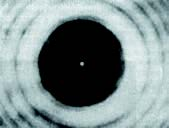
\includegraphics{6-8.pdf}
  \caption{}\label{fig:6-8}
\end{figure}

\cref{fig:6-8} 所示的圆盘可以绕通过中心 $O$ 并垂直于盘面的轴转动。
使圆盘在力 $F_1$、$F_2$ 和 $F_3$ 作用下处于平衡状态。
量出这三个力的力臂 $L_1$、$L_2$ 和 $L_3$。
分别计算出它们的力矩 $M_1 =F_1 L_1$, $M_2 =F_2 L_2$,$M_3 =F_3 L_3$,可以发现,使圆盘向顺时针方向转动的力矩之和等于使圆盘向反时针方向转动的力矩之和,即
\[M_1+M_2=M_3.\]

改变力和力臂,再做这个实验,可以得到同样的结果。
在有固定转动轴的物体上,如果所有向时针方向转动的力矩之和等于所有向反时针方向转动的力矩之和,或者考虑到力矩的正负,所有力短的代数和为零,那么,物体将处于平衡状态。

结论:\emph{有固定转动轴的物体的平衡条件是力矩的代数和等于零}。即
\[M_1+M_2+M_3\cdots=0, \]
或者
\[M_{\text{合}}=0.\]

\begin{Practice}
\begin{question}
  \item 当我们开关门窗时,如果力的作用线通过转轴,无论多大的力也不能把门窗打开或关上,为什么?
  \item 如\cref{fig:6-9} 所示,如在自行车脚踏板上的向下的力是 \qty{15}{N},求这个力的力矩。
  \begin{figurehere}
  \begin{minipage}[b]{0.58\linewidth}\centering
    \includegraphics[scale=.85]{6-9.pdf}
    \caption{}\label{fig:6-9}
  \end{minipage}
  \begin{minipage}[b]{0.38\linewidth}\centering
    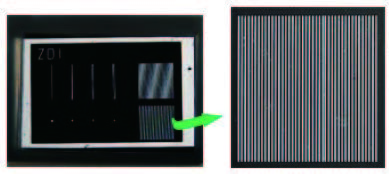
\includegraphics{6-10.pdf}
    \caption{}\label{fig:6-10}
  \end{minipage}
  \end{figurehere}
  \item \cref{fig:6-10} 是汽车制动器的路板的示意图。$O$ 是转动轴,$B$ 端连接制动器。如果司机踏紧踏板的力 $F$ 为 \qty{20}{N},制动器的阻力 $F'$ 是多大?
  \item 试根据有固定转动轴的物体的平衡条件来证明初中学过的杠杆的平衡条件:如果作用在杠杆上的两个力使杠杆向相反方向转动,并且这两个力的大小跟它们的力臂长度成反比,杠杆就平衡。
  \item 一个有固定转动轴的物体受到四个力的作用,其中使物体向顺时针方向转动的两个力是 \qty{5}{N} 和 \qty{3}{N},使物体向反时针方向转动的两个力是 \qty{2}{N} 和 \qty{6}{N}。这四个力的力臂依次是 \qtylist{0.50;0.25;0.05;0.20}{m},在这四个力的作用下,物体能否平衡?为了使物体平衡,应该把一个 \qty{1}{N} 的力加在物体上离转动轴多远的地方?这个力的力矩是正的还是负的?
\end{question}
\end{Practice}


\section{力偶}

有固定转动轴的物体不能发生平动,只能发生转动。
如果没有固定转动轴,情况会怎样呢?
照\cref{fig:6-11} 那样,在圆盘上绕一条线,然后拉这条线,使圆盘受到力的作用,那么原来静止的圆盘就同时发生转动和平动。
能不能做到使物体不发生平动,只发生转动呢?
如果照\cref{fig:6-12} 那样,在圆盘上绕两条线,然后用大小相等方向相反的力拉这两条线,那么原来静止的圆盘就只发生转动,不发生平动。

\begin{figure}
	\begin{minipage}[b]{0.52\linewidth}\centering
    \includegraphics{6-11.pdf}
    \caption{一个力可以使物体同时发生转动和平动}\label{fig:6-11}
	\end{minipage}%
	\begin{minipage}[b]{0.48\linewidth}\centering
    \includegraphics{6-12.pdf}
    \caption{力偶使物体只发生转动}\label{fig:6-12}
	\end{minipage}
\end{figure}
\begin{figure}
  \begin{minipage}[b]{0.41\linewidth}\centering
		\includegraphics{6-13.pdf}
		\caption{两手对方向盘产生一个力偶}\label{fig:6-13}
	\end{minipage}
	\begin{minipage}[b]{0.57\linewidth}\centering
		\includegraphics{6-14.pdf}
    \caption{用套筒拧螺母,两手对套筒产生一个力偶}\label{fig:6-14}
	\end{minipage}
\end{figure}

两个大小相等方向相反而在同一直线上的力,叫做\Concept{力偶}。
\emph{力偶的作用是使物体只发生转动}。
在实际上常常利用力偶来使物体转动。
用两手转动汽车的方向盘(\cref{fig:6-13}),用两手转动套筒(\cref{fig:6-14}),拿钥匙开锁,用螺丝刀拧螺丝钉,都是常见的例子。

对有固定转动轴的物体来说,用一个力可以使它转动,用两个力组成力偶也可以使它转动。
例如\cref{fig:6-14} 中不用两只手扳,用一只手扳,也可以使套简转动,但这两种情况还是不同的。
从\cref{fig:6-11} 所示的实验知道,一个力作用在物体上,可以同时产生转动作用和平动作用。
一个力作用在有固定转动轴的物体上,物体所以没有发生平动,是因为物体受到固定转动轴的限制,这时转动物体要受到转动轴的压力,转动轴同时也要受到转动物体的压力。
这种压力往往是不利的,例如用一只手扳套筒,就容易磨损螺纹。
用力偶来使物体转动,因为力偶只产生转动作用,在转动物体和转动轴之间就不会产生压力。
因此,如果希望只产生转动作用,那就应该用力偶来使物体转动。

\medskip\noindent
\begin{minipage}{0.55\linewidth}\parindent2em
我们知道,力对物体的转动作用决定于力矩。
所以力偶的转动作用决定于它的两个力的力矩的代数和。
从\cref{fig:6-15} 可以知道,力偶的两个力对任一点 $O$ 的力矩的代数和是 $M=FL+F(d-L)=Fd$。其中 $d$ 是力偶的两个力之间的垂直距离,叫做\Concept{力偶臂}。
力偶的一个力和力偶臂的乘积 $Fd$ 叫做\Concept{力偶矩}。
从上面的讨论知道,力偶的转动作用决定于力偶矩。
\end{minipage}\hfill
\begin{minipage}{0.4\linewidth}\centering
  \begin{figurehere}
    \includegraphics{6-15.pdf}
    \caption{}\label{fig:6-15}
  \end{figurehere}
\end{minipage}

\medskip
跟力矩一样,力偶矩可以使物体向不同的方向转动。
一般也是规定使物体向反时针方向转动的力偶矩是正的,使物体向顺时针方向转动的力偶矩是负的。
\cref{fig:6-15} 中的力偶矩是正的。

如果有几个力偶作用在物体上,那么这几个力偶共同对物体的转动作用决定干它们的力偶矩的代数和。
力偶矩的代数和不等于零,角速度将发生改变,物体做变速转动;力偶矩的代数和等于零,物体将用原来的角速度转动或者保持静止。
因此,在力偶作用下物体的平衡条件是力偶矩的代数和等于零。

\begin{Practice}
\begin{question}
    \item 在\cref{fig:6-13} 中,汽车方向盘的半径是 \qty{0.20}{m},司机两手加在方向盘上的力都是 \qty{15}{N},求方向盘受到的力偶矩。
    \item 一个物体受到两个力偶的作用,力偶矩的代数和 \qty{50}{N.m},这两个力偶的四个力的力矩的代数和是多大?
    \item 一个物体受到三个力偶的作用,其中两个使物体向顺时针转动的力偶的力分别是 \qty{3}{N} 和 \qty{4}{N} ,力偶臂分别是 \qty{0.50}{m} 和 \qty{0.25}{m} ;另一个使物体向反时针转动的力偶的力是 \qty{5}{N},力偶臂是 \qty{0.50}{m},这个物体能够平衡吗?
\end{question}
\end{Practice}

\section{平衡的种类}
一只茶杯很容易放在桌面上保持平衡。
这时茶杯受到竖直向下的重力和竖直向上的支持力,二者大小相等方向相反,茶杯处于平衡状态。
把铅笔削尖,使铅笔尖端朝下立在桌面上保持平衡,从道理上讲是可以实现的。
只要使铅笔所受重力的作用线绝对准确地通过铅笔尖跟桌面接触的那一点,从而使重力和支持力大小相等方向相反而且作用在一条直线上,铅笔就处于平衡位置,就应该立得住。
道理上是如此,事实上却很难实现。
我们很难使铅笔绝对准确地处在平衡位置;即使千方百计使铅笔达到了平衡位置,也避免不了各种各样的偶然因素,如微风的吹拂或桌面的轻微振动,使铅笔稍微偏离平衡位置,而且一旦偏离这个位置,在重力的作用下偏离就会越来越大,铅笔就要倾倒。
茶杯在桌面上的平衡,铅笔尖端朝下立在桌面上的平衡,这两种情况显然不同。
通常我们说前者的平衡是稳定的,后者的平衡是不稳定的。
同样是达到了平衡,还有一个平衡是否稳定的问题。
\begin{figure}
  \includegraphics{6-16.pdf}
  \caption{有支点的物体的平衡}\label{fig:6-16}
\end{figure}

\cref{fig:6-16} 表示放在凹面底部、凸面顶部和平面上的小球,它们所受的重力和支持力大小相等方向相反,都处在平衡位置。
前面说过,各种各样的偶然因素会使物体稍微偏离平衡位置,使平衡遭到破坏。
我们研究平衡是否稳定,就是要看平衡遭到破坏之后,物体是否能够回到原来的平衡位置。放在凹面底部的小球稍微偏离平衡位置之后,小球的重心升高,重力和支持力不再保持平衡,重力的作用是使小球回到平衡位置,恢复平衡。
从\cref{fig:6-16} 看出,这时重力和支持力的合力是指向平衡位置的,这种平衡叫做\Concept{稳定平衡}。
放在凸面顶部的小球稍微偏离平衡位置之后,小球的重心降低,重力和支持力也不再保持平衡,重力的作用是使小球继续远离原来的位置而不能恢复平衡。
从\cref{fig:6-16} 看出,这时重心和支持力的合力是指向远离平衡位置的方向的,这种平衡其实很难实现,叫做\Concept{不稳平衡}。
平面上的小球偏离原来的位置之后,重心的高度不变,重力和支持力依然保持平衡,也就是说,小球在平面的任何位置都能平衡。
这种平衡叫做\Concept{随遇平衡}。

上面讨论了有支点的物体的平衡,这对有支轴的物体的平衡也是正确的。
\cref{fig:6-17} 表示有支轴的物体的三种平衡情况。
在这三种情况中重力的作用线都通过支轴,力矩为零,物体都处于平衡位置。
在第一种情形里,物体的重心在支轴的正下方,物体稍微偏离平衡位置之后,重心升高,重力的力矩将使物体回到原来的位置,恢复平衡,因而属于稳定平衡。
在第二种情形里,物体的重心在支轴的正上方,稍微偏离平衡位置之后,重心降低,重力的力矩将使物体继续远离原来的位置而不能恢复平衡,这种平衡也很难实现,属于不稳平衡。
在第三种情形里,物体的重心就在支轴上,物体偏离原来的位置之后,重心的高度不变,重力的力矩仍旧为零,物体在任何位置都能平衡,因而属于随遇平衡。
\begin{figure}
  \includegraphics{6-17.pdf}
  \caption{有支轴的物体的平衡}\label{fig:6-17}
\end{figure}

从上面的讨论可以得到结论:在重力和支持力作用下处于平衡的物体,在稍微偏离平衡位置之后,如果重心升高,平衡就是稳定平衡;如果重心降低,平衡就是不稳平衡;如果重心的高度不变,平衡就是随遇平衡。

\section{稳度}
各种建筑物,工厂的烟囱,桌子、椅子、柜橱等家具,都是有支面的物体。
有支面物体的平衡是稳定平衡。
这是因为物体稍微偏离平衡位置,它的重心总要升高,重力的作用线还会通过支面,重力对作为转动轴的 $O$ 轴的力矩将使物体回到原来的位置,恢复平衡。
只有偏离平衡位置大一些,重力的作用线不再通过支面,重力的力矩才会使物体继续远离原来的位置而倾倒(\cref{fig:6-18})。
\begin{figure}
\begin{minipage}[b]{0.4\linewidth}\centering
  \includegraphics{6-18a.pdf}
  \subcaption{}\label{fig:6-18a}
\end{minipage}
\begin{minipage}[b]{0.4\linewidth}\centering
  \includegraphics{6-18b.pdf}
  \subcaption{}\label{fig:6-18b}
\end{minipage}
\caption{有支面的物体的平衡}\label{fig:6-18}
\end{figure}

平放的砖和竖放的砖都处于稳定平衡,它们是不是还有什么区别呢?
区别在于它们稳定程度不同,竖放的砖容易使它的重力作用线超出支面,容易倾倒,稳定程度较小;平放的砖不容易使它的重力作用线超出支面,不容易倾倒,稳定程度较大。

稳定程度的大小通常用\Concept{稳度}来表示。
稳度的大小跟物体重心的高低和支面的大小都有关系。

拿两个支面大小相同而重心高度不同的长方体来,如果使它们倾斜某一相同的角度(\cref{fig:6-19}),可以看到:重心低的长方体的重力作用线可以仍旧通过支面,而重心高的长方体的重力作用线不再通过支面。
可见,物体的重心越低,稳度越大。
\begin{figure}
  \includegraphics{6-19.pdf}
  \caption{重心越低,稳度越大}\label{fig:6-19}
  \includegraphics{6-20.pdf}
  \caption{支面越大,稳度越大}\label{fig:6-20}
\end{figure}

再拿两个重心高度相同而支面大小不同的长方体来。
如果使它们倾斜某一相同的角度(\cref{fig:6-20}),可以看到:支面大的长方体的重力作用线可以仍旧通过支面,而支面小的长方体的重力作用线不再通过支面。
可见,物体的支面越大,稳度越大。

这里应该说明一下,所谓支面不一定如同长方体那种情形是指长方体跟支持物的实际接触面。
桌子是四条腿着地的,桌子的支面是指四条桌腿所围成的矩形;三角架是三条腿着地的,它的支面是指以这三条腿为顶点所围成的三角形(\cref{fig:6-21})。

\medskip\noindent
\begin{minipage}{0.71\linewidth}\parindent2em
增大物体的稳度在实际中有重要意义。
为了增大物体的稳度,可以降低重心的高度或者增大支面的面积,也可以同时降低重心的高度和增大支面的面积。
许多机器、仪器、设备不能做得“头重脚轻”,而要做得底部较重底座较大,如实验用的天平安置在支面较大而且较重的底座上,实验用的铁架有一个支面较大的铸铁座,都是为了增大稳度。
设计汽车、电车等交通工具,要考虑到尽可能降低重心的高度。
装载车船,要把重货放下面,轻货放上面,使重心降低。
照相机和某些测量仪器安置在支面相当大的三角架上,高压电线的铁塔有相当大的支面,都是为了增大稳度。
\end{minipage}\hfill
\begin{minipage}{0.27\linewidth}\centering
  \begin{figurehere}
    \includegraphics{6-21.pdf}
    \caption{三角架的支面}\label{fig:6-21}
  \end{figurehere}
\end{minipage}

\begin{Practice}
\begin{question}
  \item 背上背着重东西的人,为什么要向前倾?
  \item 老年人扶手杖走路为什么不容易跌倒?
  \item 用载重汽车装运木箱,一些木箱装的是铁钉,另一些木箱装的是铝制器皿,怎祥装木箱,汽车的稳度比较大?
  \item 下列情况是哪类平衡?
  \begin{tasks}(2)
    \task 体操运动员在吊环上做倒立;
    \task 体操运动员吊在吊环上;
    \task 杂技演员走钢丝;
    \task 轮子套在水平轴上。
  \end{tasks}
  \item 把一个长方体立在一块木板上,在长方体前表面的中心点固定一个小螺钉,在小螺钉上拴一个小铅锤。把木块的一端慢慢抬起,研究一下长方体在什么条件下才倾倒?已知前表面的边长,你能否算出木块要抬起多大角度,长方体才倾倒?实际算一算,再用实验来检验。
\end{question}
\end{Practice}

\begin{Review}
\begin{question}
  \item 在共点力作用下物体的平衡条件是什么?
  \item 什么叫做力矩?力对物体的转动作用决定于什么?
  \item 有固定转动轴的物体的平衡条件是什么?
  \item 什么叫做力偶?力偶的作用是什么?什么叫做力偶矩?力偶的转动作用决定于什么?
  \item 在重力和支持力作用下物体的平衡有哪几种?这几种平衡有什么区别?
  \item 什么叫稳度?稳度跟什么有关系,是怎样的关系?怎样增大物体的稳度?举出一些实例来。
\end{question}
\end{Review}

\begin{Exercise}
\begin{question}
  \item \cref{fig:6-22} 表示一种简易起重机,$OA$ 是钢绳,跟水平方向成 \ang{30} 角,$OB$ 是撑杆,跟水平方向成 \ang{60} 角,提起的货物重 \qty{5e3}{N}。求钢绳对货物的拉力和撑杆对货物的支持力。
  \begin{figurehere}
    \begin{minipage}[b]{0.38\linewidth}
      \centering
      \includegraphics{6-22.pdf}
      \caption{}\label{fig:6-22}
    \end{minipage}%
    \begin{minipage}[b]{0.3\linewidth}
      \centering
      \includegraphics{6-23.pdf}
      \caption{}\label{fig:6-23}
    \end{minipage}%
    \begin{minipage}[b]{0.3\linewidth}
      \centering
      \includegraphics{6-24.pdf}
      \caption{}\label{fig:6-24}
    \end{minipage}
  \end{figurehere}
% \begin{figurehere}
%   \begin{minipage}{\linewidth}\centering
%     \includegraphics{6-22.pdf}
%     \caption{}\label{fig:6-22}
%   \end{minipage}
% \end{figurehere}
% \begin{solution}
% 取$O$点作为受力点,$O$点受到三个力:货物的拉力
% $F$(等于货物的重量),钢绳的拉力$F_1$,撑杆的支持力$F_2$。$O$点在这三个力的作用下保持平衡。

% 应用平行四边形法则求出力$F_1$和$F_2$的合力$F'$。从平
% 衡条件知道,力$F'$应该与$F$大小相等方向相反。从学过的几何知识可以证明,$\triangle OF'F_1$是等腰三角形,它的两个等角是30$^\circ$。

% 应用等腰三角形的性质可以求出$F_1$:$F_1=F'=F$。即$F_1=5.0\times 10^3$牛。

% 应用正弦定理则可以求出$F_2$:
% \[\begin{split}
% \frac{F_2}{F}&=\frac{\sin 120^{\circ}}{\sin 30^{\circ}}\\
% F_2&=\frac{\sin 120^{\circ}}{\sin 30^{\circ}}F=8.5\times 10^3 {\rm N}
% \end{split}\]
% 这个题也可以用力的分解来求解。但是求解物体平衡的问题,一般还是应用平衡条件为好,因为不管受力情况怎样复杂,平衡条件都适用。
% \end{solution}

\item \cref{fig:6-23} 中的 $AC$ 和 $BC$ 是固定在电线杆上的铁棍,$AC$ 长 \qty{0.9}{m},$BC$长 \qty{1.2}{m},$AB$ 之间的距离是 \qty{0.6}{m},在 $C$ 处挂一盏重 \qty{20}{N} 的街灯,求 $AC$ 对街灯的拉力和 $BC$ 对街灯的支持力。
\item \cref{fig:6-24} 中的 $BO$ 是一根横梁,一端安在轴 $B$ 上,另一端用钢绳 $AO$ 拉着,在 $O$ 点挂一个重物,重量是 \qty{240}{N}。横梁是均匀的,它本身的重量是 \qty{80}{N}。求钢绳的拉力。

% \begin{solution}
%     取横梁$BO$作为研究对象,横梁的一端安在轴$B$上,是一个有固定转动轴的物体。力$F$的力矩是$Fl$,力$T$的力矩是$Tl\sin\theta$,自重$G$的力矩是$Gl/2$。应用有固定转动轴物体的平衡条件得到:
% \[    Tl\sin\theta -G\frac{l}{2}-Fl=0,\]
% \[T= \frac{G+2F}{2\sin\theta }=560{\rm N}\]

% 在这个题里,如果把力$F$沿$AO$和$OB$方向分解来求钢绳
% 的拉力,就会得到错误的结果。因为对钢绳的拉力$T$不仅跟物体的重量有关,而且跟横梁的自重有关。这时力$F$在$AO$方
% 向的分力没有实际意义。
% \end{solution}

\item 一根木料,抬起它的右端要用 \qty{480}{N} 竖直向上的力,抬起它的左端要用 \qty{650}{N} 竖直向上的力,这根木料有多重?
\item 放在斜面上的一个物体,当斜面倾角为 $\theta$ 时,它沿着斜面匀速下滑。试证明物体和斜面之间的滑动摩擦系数 $\mu=\tan \theta$。
\item 如果天平的两臂并不完全相等,可以采取所谓复称法求得物体的真实质量 $m$。先把物体放在左盘,砝码放在右盘,天平平衡时砝码的质量是 $m_1$。然后把物体放在右盘,砝码放在左盘,天平平衡时砝码的质量是 $m_2$。试证明物体的真实质量 $m=\sqrt{m_1m_2}$。
\item 无风的时候竖直下落的雨滴受到两个力的作用:重力、空气阻力。设空气阻力 $f$ 与雨滴下落的速度 $v$ 成正比,即 $f=kv$。开始下落时雨滴的速度较小,空气阻力也较小,雨滴加速下落,速度随来越大。随着速度的增大,空气阻力也增大,当空气阻力增大到与重力平衡时,雨滴就以一定的速度匀速下落。这个速度叫做极限速度或收尾速度,设雨滴的质量为 $m$,试证明雨滴的极限速度 $v=mg/k$。
\item 降落伞由于受到水平方向的风力而沿着跟竖直方向成 \ang{30} 角的方向匀速下降,降落伞和人共重 \qty{700}{N},求降落伞所受的空气的阻力。
\item \cref{fig:6-25} 是一台起重机的示意图,机身和平衡体的重量 $G_1=\qty{4.2e5}{N}$,起重杆的重量 $G_2=\qty{2.0e4}{N}$,其他数据如图中所示。起重机至多能提起多重的货物。
\begin{figurehere}
  \begin{minipage}{\linewidth}\centering
    \includegraphics{6-25.pdf}
    \caption{}\label{fig:6-25}
  \end{minipage}
\end{figurehere}
提示:这时起重机以 $O$ 为转动轴而保持平衡。

\item  \cref{fig:6-26} 是一把杆秤,提扭和挂钩的距离 $OB$ 是 \qty{6.0}{cm},秤锤的质量是 \qty{600}{g}。不称物体时,把秤锤挂在 $A$ 点,杆秤平衡,$A$ 点就是刻度的起点,设 $OA$ 为 \qty{1.6}{cm},杆秤的质量为 \qty{240}{g},求杆秤的重心。在称某一物体时,秤锤移到 $D$ 点后杆秤平衡,$AD$ 为 \qty{24}{cm},所称物体的质量是多少?
\begin{figurehere}
  \begin{minipage}{\linewidth}\centering
    \includegraphics{6-26.pdf}
    \caption{}\label{fig:6-26}
  \end{minipage}
\end{figurehere}
\item 天平的横梁(连同指针)是一个有固定转动轴的物体,转动轴就是中央刀口 $O$(\cref{fig:6-27})。横梁的自重为 $G$,重心 $C$ 在指针上离转动轴 $O$ 为 $h$ 的地方。天平两盘中的重量相等时,作用在横梁两端的力 $F$ 相等,横梁平衡,指针指在标尺的中央,即指针停在竖直方向,天平两盘中的重量稍有不等,横梁就要倾斜,指针随着偏移到较轻的一方,自重 $G$ 对转动轴 $O$ 的力矩将阻止横梁倾斜,最后横梁在某一倾斜位置上达到平衡。设指针与竖直方向成 $\theta$ 角时横梁平衡,可以证明
\[\tan\theta =\frac{L}{Gh}(F_1-F_2).\]
从上式可以看出,对于天平两盘中一定的重量差,$G$ 和 $h$ 越小,则 $\theta$ 角越大,这种天平越灵敏。所以通常灵敏的天平要选用轻质材料做横梁,并要提高重心的高度。
\begin{figurehere}
  \begin{minipage}{\linewidth}\centering
    \includegraphics{6-27.pdf}
    \caption{天平的平衡}\label{fig:6-27}
  \end{minipage}
\end{figurehere}
试应用有固定转动轴的物体的平衡条件证明上式。

\item  \cref{fig:6-28} 表示拖拉机(或汽车)在上坡。拖拉机前后轮的轮距是 $L$,重心的高度是 $h$,重心至前轮的距离是 $l$。可以证明,上坡时不致向后翻倒,路面的最大倾角 $\theta_1$ 满足条件:
\[\tan\theta_1=\frac{L-l}{h}.\]
\begin{figurehere}
  \begin{minipage}{\linewidth}
    \centering\includegraphics{6-28.pdf}
    \caption{}\label{fig:6-28}
  \end{minipage}
\end{figurehere}
拖拉机下坡时,可以证明,下坡时不致向前翻倒,路面的最大倾角 $\theta_2$ 满足条件:
\[\tan\theta_2=\frac{l}{h}.\]
试证明上两式,并根据上两式讨论:重心太高、太靠前、太靠后有什么不好?
\end{question}
\end{Exercise}
